
\documentclass[a4paper,11pt,final,oneside,openright]{book}
\usepackage{rapport}

\newcommand{\reporttitle}{Développement Orienté Objet}
\newcommand{\enseignants}{Christine~\textsc{Solnon}\\ Elöd~\textsc{Egyed-Zsigmond}}
\newcommand{\reportauthor}{Guillaume~\textsc{Abadie}\\ Nicolas~\textsc{Buisson}\\ Louise~\textsc{Crépet}\\ Rémi~\textsc{Domingues}\\ Aline~\textsc{Martin}\\ Martin~\textsc{Wetterwald}}
\newcommand{\hexanome}{H4404}
\newcommand{\reportsubject}{Livrable de projet}
\newcommand{\dateperiod}{du 27 novembre au 20 décembre 2013}
\newcommand{\HRule}{\rule{\linewidth}{0.5mm}}
\setlength{\parskip}{1ex} % Espace entre les paragraphes

\hypersetup{
    pdftitle={\reporttitle},%
    pdfauthor={\reportauthor},%
    pdfsubject={\reportsubject},%
    pdfkeywords={INSA Lyon} {mot1} {mot2} {mot3}
}

\title{\reporttitle}
\author{\reportauthor}

%\setcounter{tocdepth}{4}
\begin{document}
    \renewcommand{\chaptername}{} %\renewcommand{\thechapter}{}
    \renewcommand{\contentsname}{Sommaire}

	\glsaddall
	\renewcommand{\chaptername}{}
	\renewcommand{\glossaryname}{Glossaire}

    \pagestyle{empty}
    \pagenumbering{Roman}
    % Inspiré de http://en.wikibooks.org/wiki/LaTeX/Title_Creation
\begin{center}
	\begin{minipage}[t]{0.48\textwidth}
	  \begin{flushleft}
	    
\includegraphics [width=40mm]{images/logo_INSA.png} \\[0.5cm]
			INSA Lyon\\
			20, avenue Albert Einstein\\
			69621 Villeurbanne Cedex
	  \end{flushleft}
	\end{minipage}
	\begin{minipage}[t]{0.48\textwidth}
	  \begin{flushright}
	    %\includegraphics [width=60mm]{images/logo_Passau.jpg} \\[0.5cm]
	    %Universität Passau\\
		%Innstraße, 3\\
		%	D-94032 Passau
	  \end{flushright}
	\end{minipage} \\[2cm]

	\textsc{\Large \reportsubject}\\[0.3cm]
	\HRule \\[0.4cm]
	{\Huge \bfseries \reporttitle}\\[0.6cm]
	{\Large \dateperiod}\\[0.4cm]
	\HRule \\[1cm]

	
\includegraphics [scale=0.55]{images/livraison.jpg} \\[0.7cm]
	\begin{minipage}[t]{0.4\textwidth}
	  \begin{flushleft} \large
	    \emph{Hexanôme \textbf{\hexanome}~:}\\
	    \small \reportauthor
	  \end{flushleft}
	\end{minipage}
	\begin{minipage}[t]{0.5\textwidth}
	  \begin{flushright} \large
	    \emph{Enseignants~:} \\
	    \enseignants
	  \end{flushright}
	\end{minipage}

	\vfill
	\footnotesize{Année scolaire 2013-2014}
\end{center}

    \sloppy          % Justification moins stricte : des mots ne dépasseront pas des paragraphes

    \frontmatter
    \pagestyle{empty}
    \tableofcontents
    \addtocontents{toc}{\protect\thispagestyle{empty}}

    \mainmatter
    \pagestyle{headings}
	\renewcommand{\chaptermark}[1]{\markboth{\MakeUppercase{#1}}{}}
	\renewcommand{\sectionmark}[1]{\markright{#1}}
	\chapter*{Introduction}
\addcontentsline{toc}{chapter}{Introduction}
\chaptermark{Introduction}

Ce dossier a pour but de vous présenter le sytème de gestion des livraisons du Grand Lyon, Optifret\textunderscore COURLY.
Nous nous attarderons ici plus spécifiquement sur l'interface du superviseur, qui lui permet de gérer les demandes de
livraisons des clients utilisant le système.

Vous retrouverez dans ce dossier la démarche détaillée de la capture et de l'analyse des besoins, ainsi que la
description complète de la conception de l'application. Nous espérons que notre système Optifret\textunderscore COURLY vous donnera
une entière satisfaction.



    \renewcommand{\chaptermark}[1]{\markboth{\MakeUppercase{\chaptername\ \thechapter.\ #1}}{}}
    \renewcommand{\sectionmark}[1]{\markright{\thesection{} #1}}

    \chapter{Capture et analyse des besoins}

\section{R\^oles}

\begin{description}
    \item[ABADIE Guillaume] Concepteur / D\'eveloppeur
    \item[BUISSON Nicolas] Concepteur / D\'eveloppeur
    \item[CREPET Louise] Concepteur / D\'eveloppeur
    \item[DOMINGUES R\'emi] Chef de projet / Concepteur / D\'eveloppeur
    \item[MARTIN Aline] Responsable qualit\'e / Concepteur / D\'eveloppeur
    \item[WETTERWALD MARTIN] Responsable Git / Concepteur / D\'eveloppeur
\end{description}

\section{Planning pr\'evisionnel du projet}

\begin{landscape}
\begin{figure}[h]
    \centering
    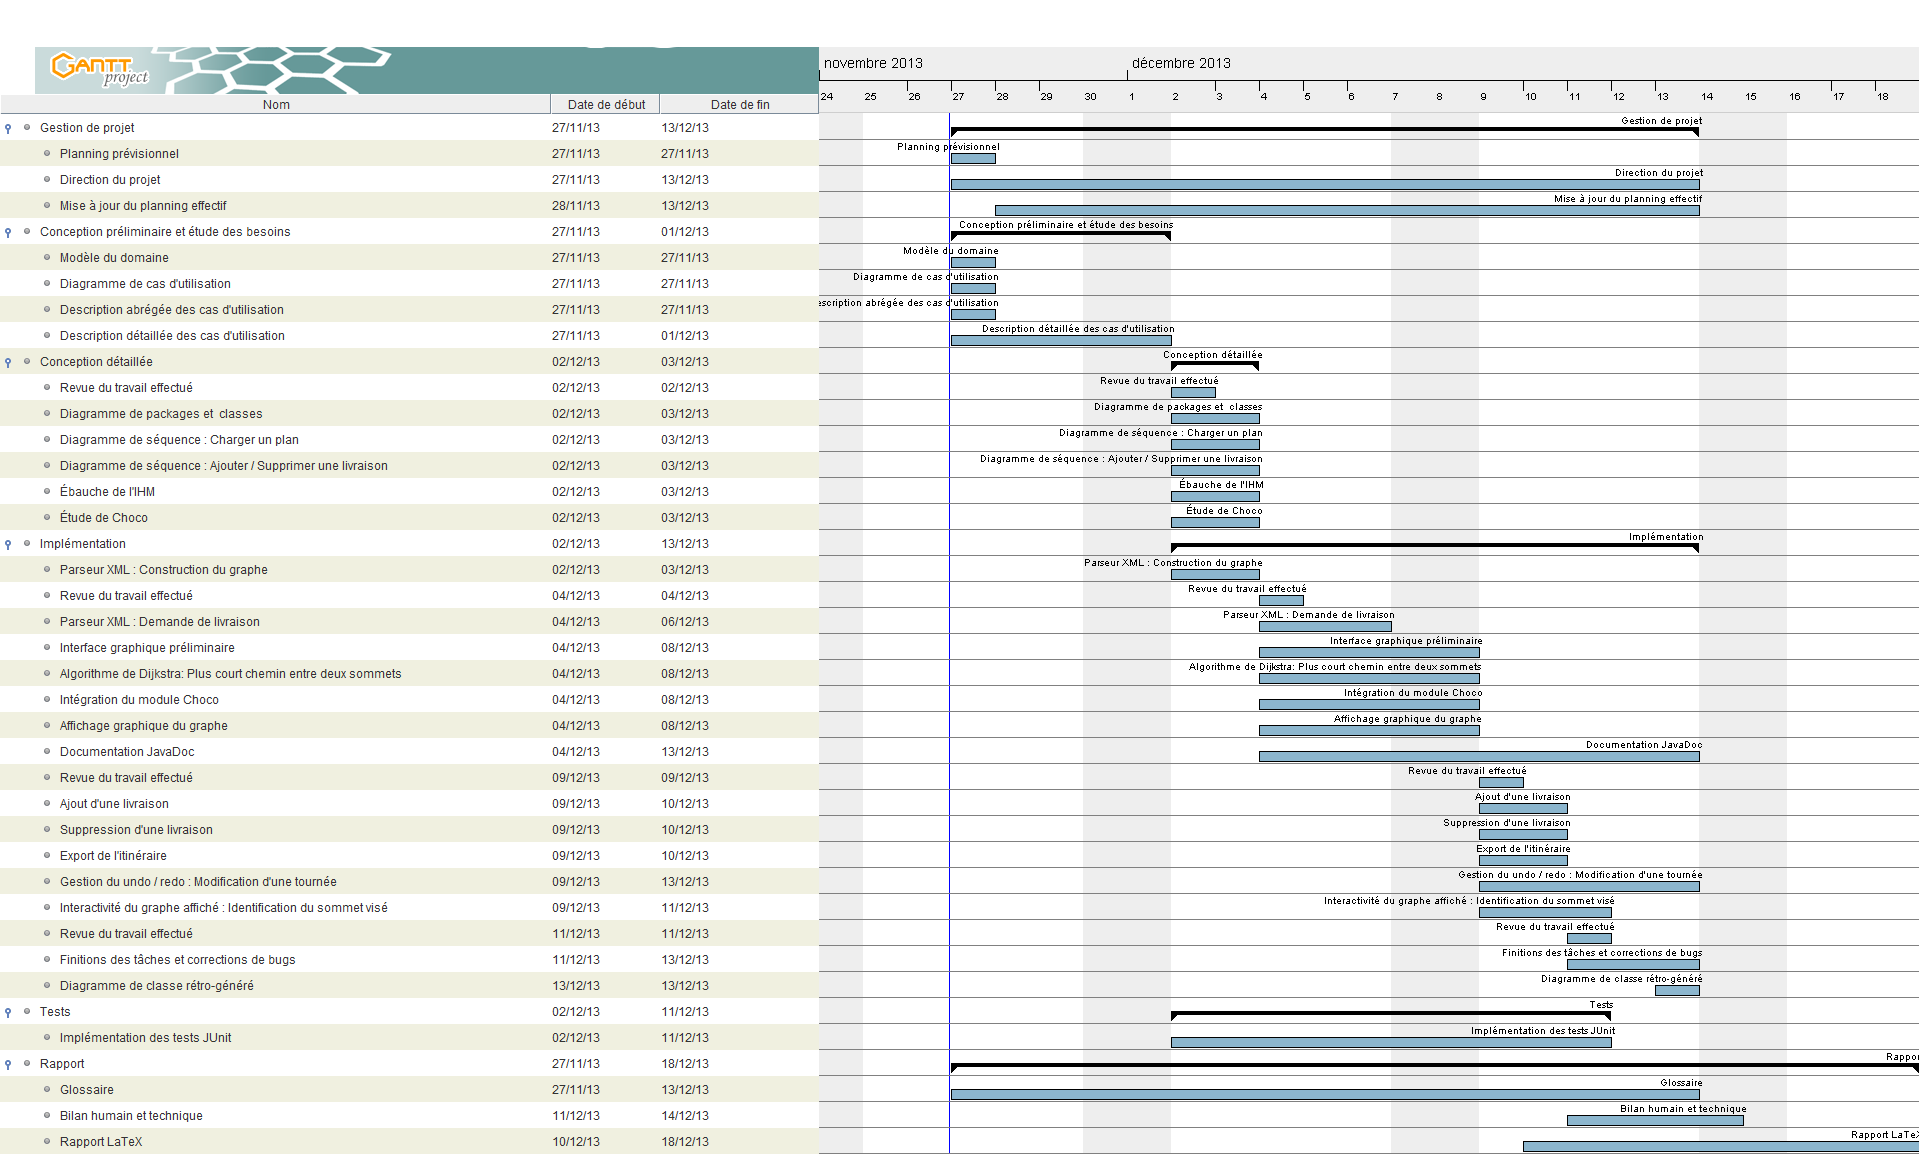
\includegraphics[width=240mm]{../diagrams/project_management/planning_previsionnel/planning_previsionnel.png}
    \caption{Planning pr\'evisionnel du projet}
    \label{diagram:planning_prevision}
\end{figure}
\end{landscape}
\pagebreak


\section{Mod\`ele du domaine}

\begin{figure}[h]
    \centering
    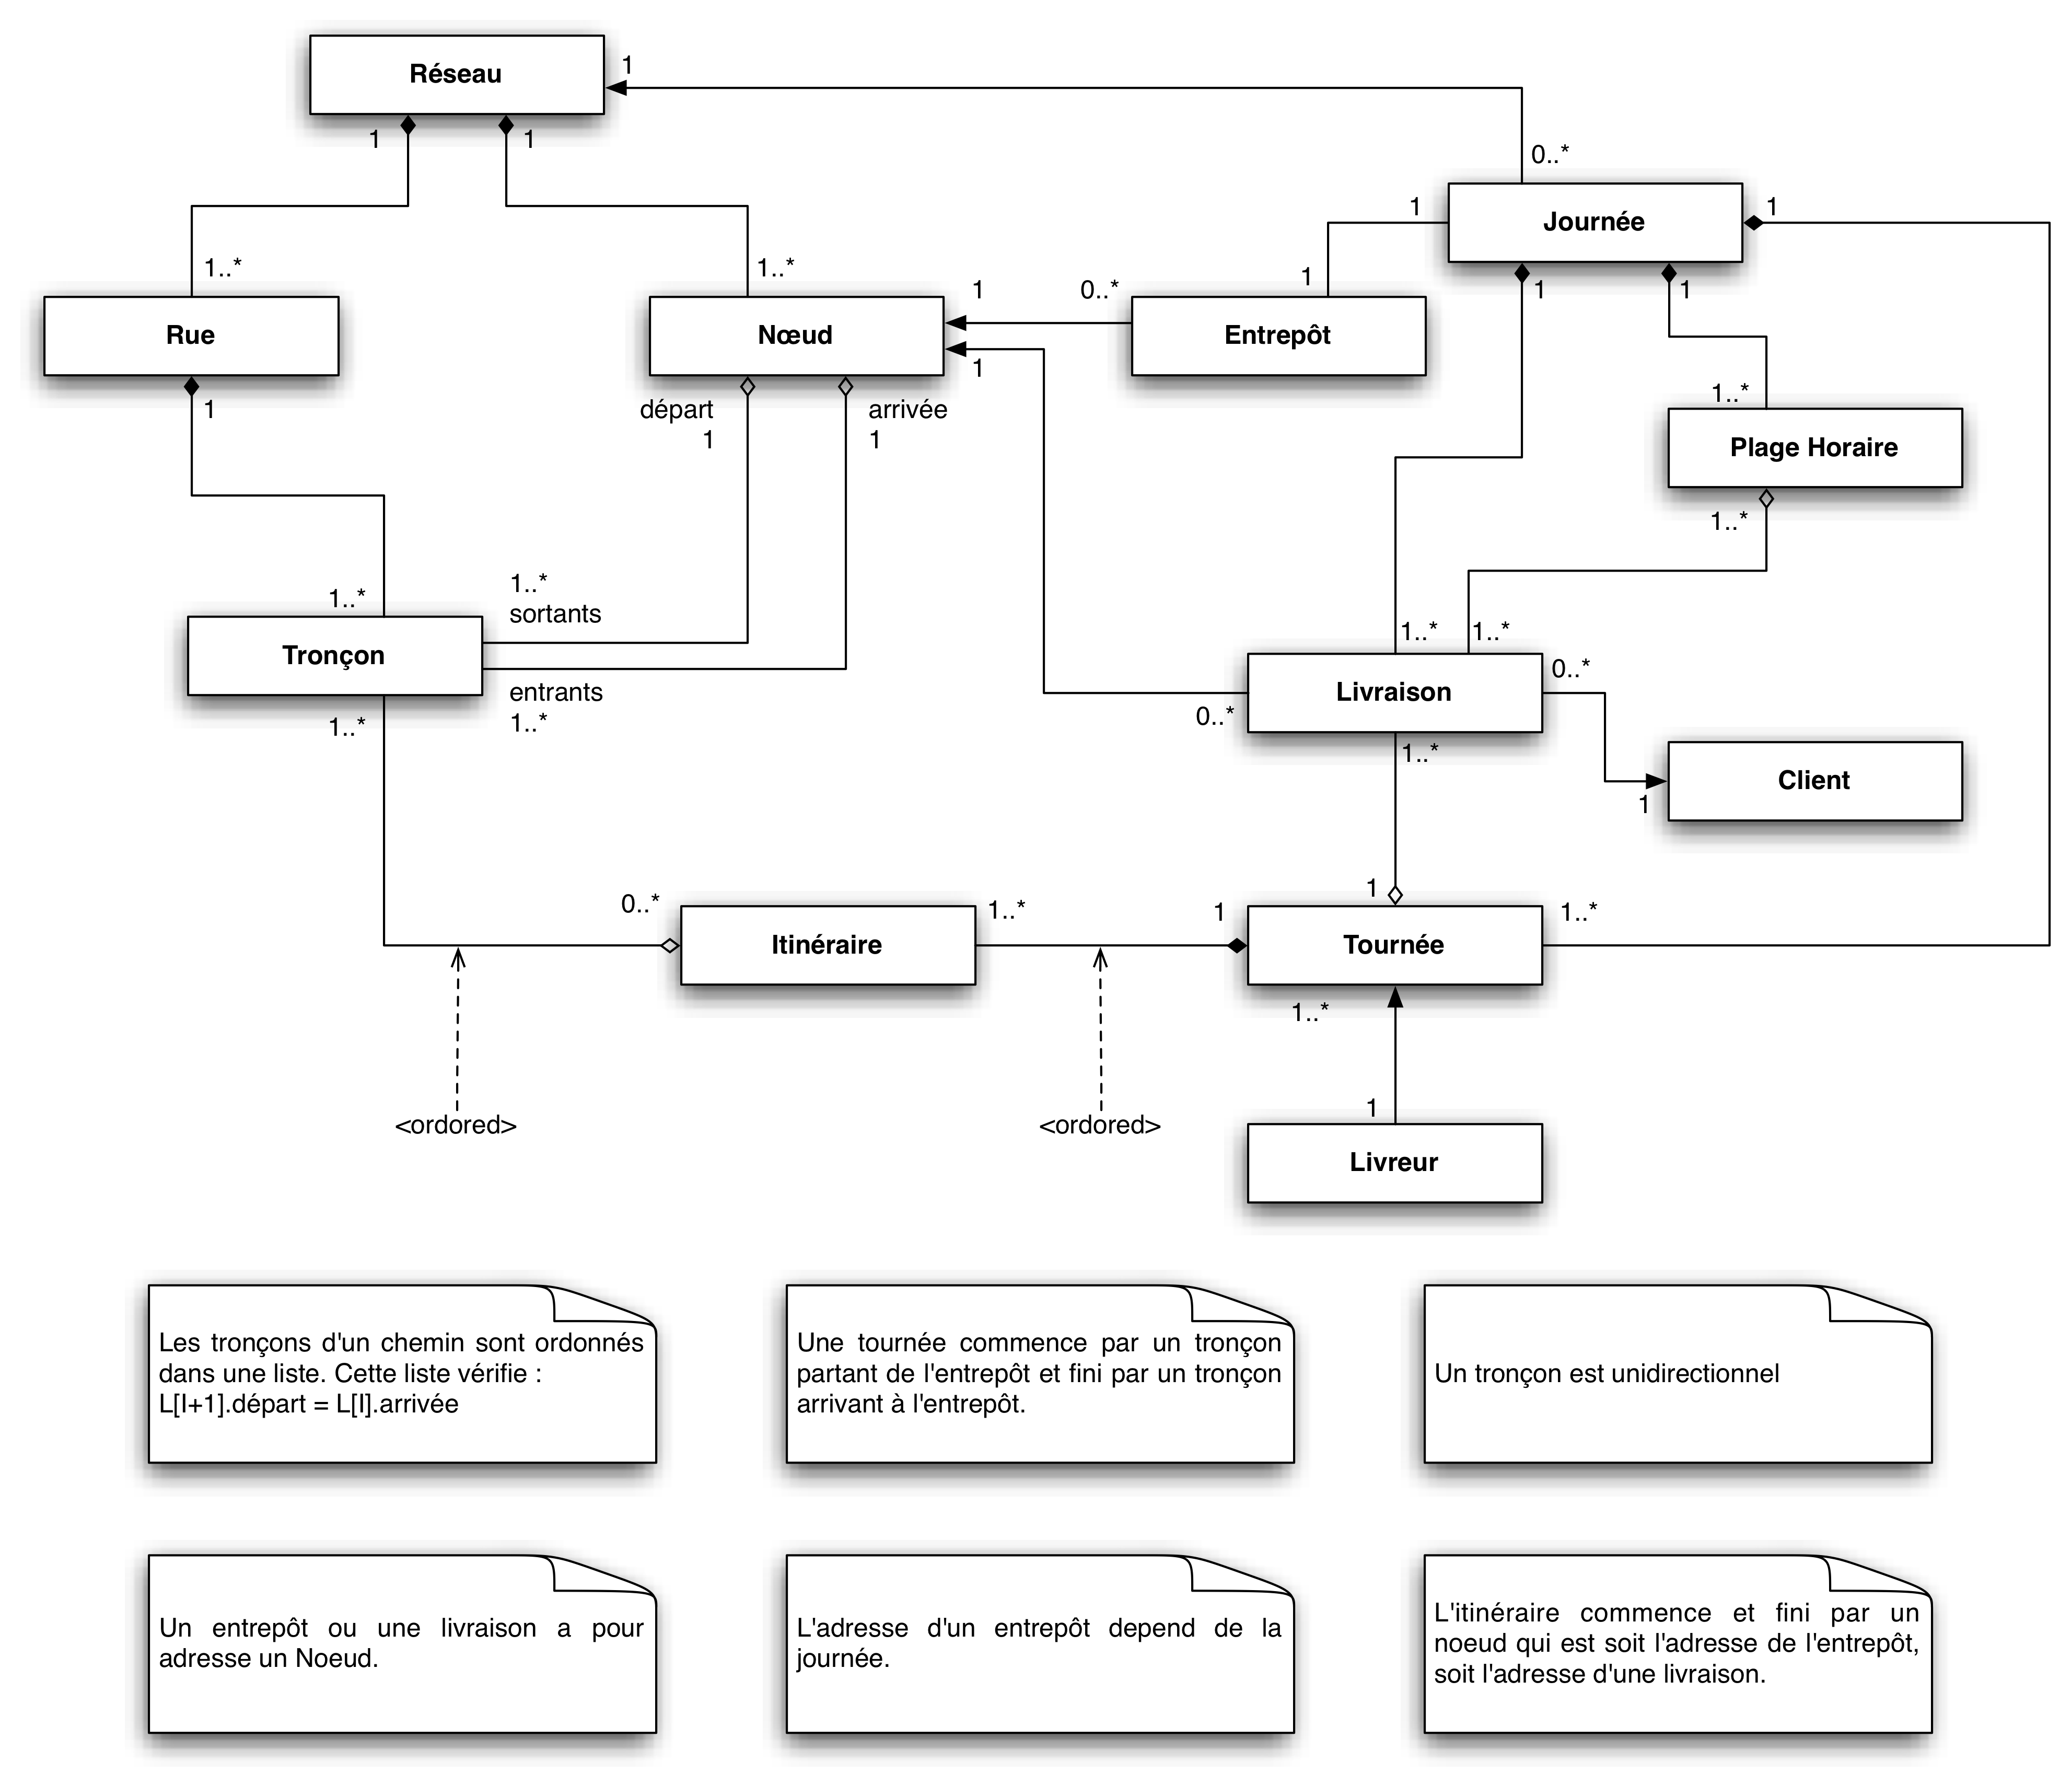
\includegraphics[width=140mm]{../diagrams/domain_model/domaine.png}
    \caption{Mod\`ele du domaine}
    \label{diagram:domaine}
\end{figure}

\pagebreak
\section{Diagramme de cas d’utilisation}

\begin{figure}[h]
    \centering
    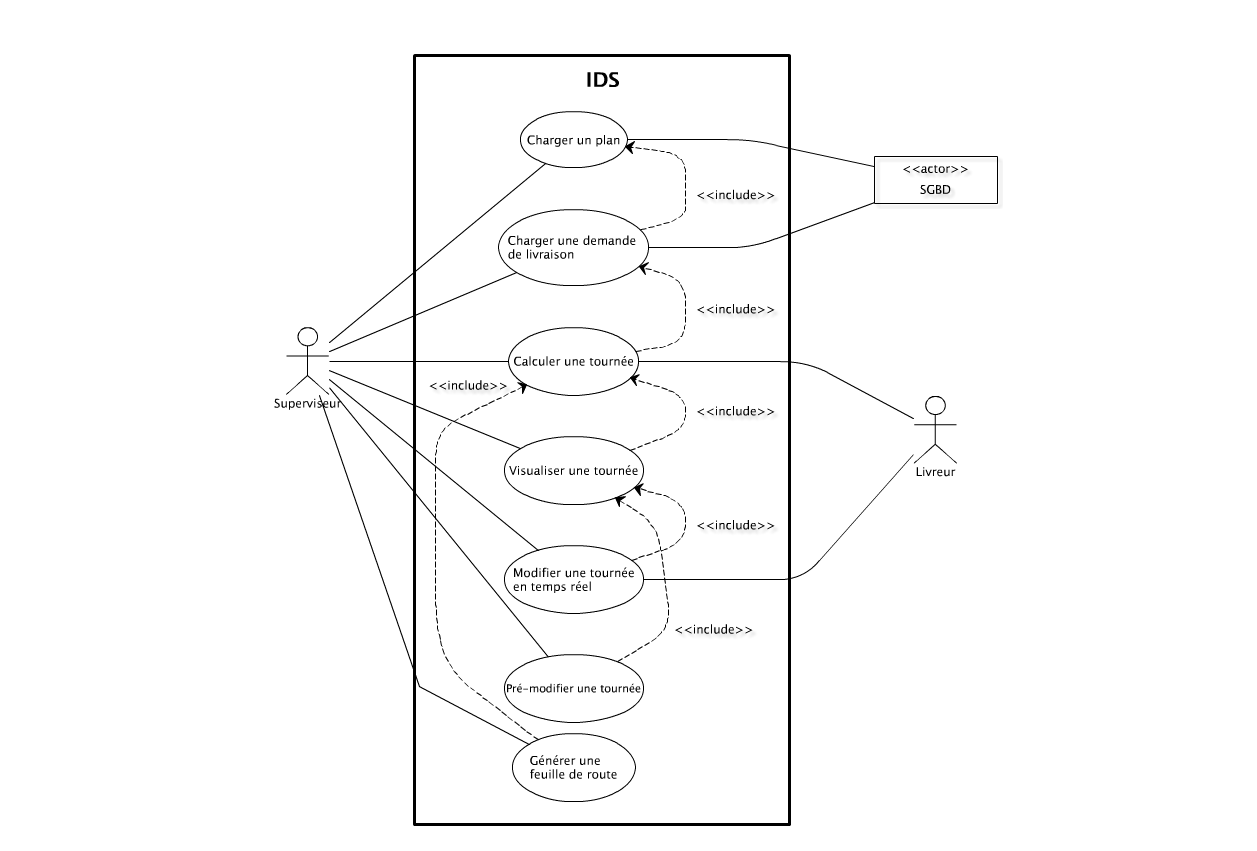
\includegraphics[width=140mm]{../diagrams/use_case/use_case_diagram.png}
    \caption{Diagramme de cas d’utilisation}
    \label{diagram:use_case}
\end{figure}

\section{Description abr\'eg\'ee des cas d’utilisation}

Le système doit permettre plusieurs ensembles d’actions~:

\begin{itemize}
    \item Le superviseur peut à tout moment visualiser le plan d’une zone de la ville, il peut alors y voir les
    points de livraison de la zone, ainsi que leur détails (adresse, état de livraison, etc …).

    \item D’autre part, il peut charger une demande de livraison, celle ci est ajoutée au système et sera traitée
    dans les futures tournées.

    \item Enfin il peut générer une feuille de route multi-support (papier et électronique) à la destination d’un
    des livreurs. Pour cela il peut demander au système de calculer une tournée, et de la visualiser sur un plan.
    Il peut alors y faire d’éventuelles modifications avant la génération de la feuille et lancer cette dernière.

    \item Une fois la feuille de route générée, le superviseur pourra à tout moment modifier une tournée en cours.
    Le livreur de cette tournée modifiée en sera alors informé par le système.
\end{itemize}


    \chapter{Conception}


% ----------------------------------------------------------------------------- Cas d'utilisations

\section{Description d\'etaill\'ee des cas d’ utilisation}

\subsection{Charger un plan}
\begin{description}
    \item[Contexte :] le superviseur veut visualiser le plan d'une zone de la ville
    \item[Acteur principal :] Superviseur
    \item[Precondition :] -
    \item[Postconditions :] Le plan doit \^etre affich\'e
    \item[Scenario principal :] ~
    \begin{enumerate}
        \item Le superviseur demande le chargement d'un plan pour une zone de la ville
        \item Le syst\`eme demande au SGBD si la zone existe bien, ainsi que les donn\`ees correspondantes
        \begin{enumerate}
            \item La zone n'existe pas :
            \begin{enumerate}
                \item Le syst\`eme renvoie une erreur, le CdU reprend \`a l'\'etape 1, le cas d'utilisation se termine par un echec.
            \end{enumerate}
            \item Erreur syntaxique, le cas d'utilisation se termine par un echec.
            \item Erreur s\'emantique, le cas d'utilisation se termine par un echec.
        \end{enumerate}
        \item Le syst\'eme affiche le plan \`a l'\`ecran, le cas d'utilisation se termine par un succ\`es.
    \end{enumerate}
\end{description}
\pagebreak

\subsection{Charger une demande de livraison}
\begin{description}
    \item[Contexte :] Le superviseur veut charger une demande de livraison, c'est-\`a-dire un ensemble de points \`a livrer avec, pour chaque point, sa
    plage horaire
    \item[Acteur principal :] Superviseur
    \item[Precondition :] Le plan doit \^etre charg\'e
    \item[Postconditions :] Les points doivent \^etre affich\'es sur le plan
    \item[Scenario principal :] ~
    \begin{enumerate}
        \item Le superviseur s\'electionne une demande de livraison
        \item Le syst\`eme demande au SGBD si la demande de livraison existe bien, ainsi que les donn\'ees correspondantes
        \begin{enumerate}
            \item La demande de livraison n'existe pas :
            \begin{enumerate}
                \item Le syst\'eme renvoie une erreur, le CdU reprend \`a l'\'etape 1, le cas d'utilisation se termine par un echec.
            \end{enumerate}
            \item Erreur syntaxique, le cas d'utilisation se termine par un echec.
            \item Erreur s\'emantique, le cas d'utilisation se termine par un echec.
        \end{enumerate}
        \item Le syst\`eme affiche les points de livraison sur le plan, le cas d'utilisation se termine par un succ\`es.
    \end{enumerate}
\end{description}

\subsection{Calculer une tourn\'ee}
\begin{description}
    \item[Contexte :] Le superviseur veut calculer une tourn\'ee pour la derni\`ere demande de livraisons charg\'ee
    \item[Acteur principal :] Superviseur
    \item[Precondition :] Une tourn\'ee doit \^etre selectionn\'ee, les demandes de livraisons doivent \^etre charg\'ees
    \item[Postconditions :] -
    \item[Scenario principal :] ~
    \begin{enumerate}
        \item Le superviseur clique sur "calculer tourn\'ee" pour la demande de livraison
        \item Le syst\`eme calcule la tourn\'ee et l'envoie au SGBD
        \begin{enumerate}
            \item Il n'est pas possible de tout faire dans les temps, le syst\`eme notifie l'utilisateur qu'il y aura forc\'ement des retards, le cas d'utilisation se termine par un succ\`es.
            \item Une livraison n'est pas accessible, le cas d'utilisation se termine par un echec.
        \end{enumerate}
        \item Le syst\`eme affiche la tourn\'ee sur le plan, le cas d'utilisation se termine par un succ\`es.
    \end{enumerate}
\end{description}
\pagebreak

\subsection{Visualiser une tourn\'ee}
\begin{description}
    \item[Contexte :] Le superviseur veut visualiser une tourn\'ee sur un plan avec les diff\'erents \'etats des livraisons (fait, \'a l'heure, en retard, etc.) Possibilit\'e de visualiser les details de la tourn\'ee.
    \item[Acteur principal :] Superviseur
    \item[Precondition :] La tourn\'ee existe et est dans une liste de tourn\'ees disponnibles
    \item[Postconditions :] La tourn\'ee existe, est dans une liste de tourn\'ees disponnibles, est selectionn\'ee et est affich\'ee
    \item[Scenario principal :] ~
    \begin{enumerate}
        \item Le superviseur clique sur la tourn\'ee dans la liste
        \item La tourn\'ee s'affiche dans la zone pr\'evue \`a cet effet
    \end{enumerate}
    \item[Extension :] ~
    \begin{enumerate}
        \item Le superviseur clique sur "d\'etail"
        \begin{enumerate}
            \item Les informations compl\'ementaires s'affichent dans la zone pr\'evue \`a cet effet, le cas d'utilisation se termine par un succ\`es.
            \item Les informations par d\'efaut s'affichent si la tourn\'ee est vide, le cas d'utilisation se termine par un succ\`es.
        \end{enumerate}
    \end{enumerate}
\end{description}

\subsection{G\'en\'erer d'une feuille de route}
\begin{description}
    \item[Contexte :] Le superviseur veut g\'en\'erer une feuille de route d'un livreur contenant les itin\'eraires de chaque livraisons
    \item[Acteur principal :] Superviseur
    \item[Precondition :] La tourn\'ee du livreur est pr\^ete.
    \item[Postconditions :] La feuille de route a \'et\'e g\'en\'er\'ee et la version papier imprim\'ee
    \item[Scenario principal :] ~
    \begin{enumerate}
        \item Le superviseur clique sur "g\'en\'erer feuille de route"
        \item La feuille de route est g\'en\'er\'ee et sauvegard\'ee, le cas d'utilisation se termine par un succ\`es.
        \begin{enumerate}
            \item Pas de livraison pour la tourn\'ee
            \item Probl\`eme avec l'ordinateur pendant la sauvegarde
            \item Le fichier existe d\'ej\`a dans les sauvegardes
            \begin{enumerate}
                \item Ecraser l'ancien, le cas d'utilisation se termine par un succ\`es.
                \item Annuler le nouveau, le cas d'utilisation se termine par un echec.
                \item Rennomer l'un des deux, le cas d'utilisation se termine par un succ\`es.
            \end{enumerate}
        \end{enumerate}
    \end{enumerate}
\end{description}
\pagebreak

\subsection{Modifier une tourn\'ee en temps r\'eel}
\begin{description}
    \item[Contexte :] Le superviseur veut modifier une tourn\'ee le jour m\^eme en ajoutant ou retirant une livraison. Il doit \^etre possible d'annuler la derni\`ere action, mais aussi de la refaire.
    \item[Acteur principal :] Superviseur
    \item[Preconditions :] ~
    \begin{description}
        \item[G\'en\'erale :] Il y a une tourn\'ee s\'electionn\'ee, il est possible de communiquer avec le livreur
        \item[Pour ajouter :] Il y a au moins un noeud libre sur le plan
        \item[Pour enlever :] Il y a au moins une livraison dans la tourn\'ee
    \end{description}
    \item[Postconditions :] ~
    \begin{description}
        \item[G\'en\'erale :] La tourn\'ee s\'electionn\'ee est modifi\'ee et les changements ont \'et\'e envoy\'es au livreur
        \item[Pour ajouter :] La livraison est ajout\'ee \`a la tourn\'ee \`a la bonne place
        \item[Pour enlever :] La livraison est enlev\'ee de la tourn\'ee qui est automatiquement recalcul\'ee
    \end{description}
    \item[Scenario principal :] ~
    \begin{description}
        \item[Ajouter] ~
        \begin{enumerate}
            \item Le superviseur selectionne un noeud disponnible
            \item Le superviseur clique sur "ajouter" et remplit le forumlaire d'ajout(plage horaire, client, etc.)
            \item Le superviseur clique sur "annuler" pendant qu'il remplit le formulaire
            \begin{enumerate}
                \item L'ajout est annul\'e et le superviseur perd ce qu'il avait pr\'e-rempli, le cas d'utilisation se termine par un echec.
            \end{enumerate}
            \item Le supervieur clique sur "ok"
            \item La livraison est ajout\'ee et la tourn\'ee recalcul\'ee
            \item L'ajout est envoy\'e au livreur, le cas d'utilisation se termine par un succ\`es.
            \begin{enumerate}
                \item La connexion au livreur \'echoue, le cas d'utilisation se termine par un echec.
            \end{enumerate}
        \end{enumerate}
        \item[Enlever] ~
        \begin{enumerate}
            \item Le superviseur selectionne une livraison sur la tourn\'ee
            \item Le superviseur clique sur "enlever"
            \item La livraison est enlev\'ee et la tourn\'ee recalcul\'ee
            \begin{enumerate}
                \item La livraison est enlev\'ee et la tourn\'ee est vide, le syst\'eme continue \`a l'\'etape enlever:4
            \end{enumerate}
            \item La suppression est envoy\'ee au livreur, le cas d'utilisation se termine par un succ\`es.
            \begin{enumerate}
                \item La connexion au livreur \'echoue, le cas d'utilisation se termine par un echec.
            \end{enumerate}
        \end{enumerate}
    \end{description}
\end{description}
\pagebreak

\subsection{Pr\'e-modifier une tourn\'ee}
\begin{description}
    \item[Contexte :] Le superviseur veut modifier une tourn\'ee la veille en ajoutant ou retirant une livraison. Il doit \^etre possible d'annuler la derni\`ere action, mais aussi de la refaire.
    \item[Acteur principal :] Superviseur
    \item[Preconditions :] ~
    \begin{description}
        \item[G\'en\'erale :] Il y a une tourn\'ee s\'electionn\'ee, il est possible de communiquer avec le livreur
        \item[Pour ajouter :] Il y a au moins un noeud libre sur le plan
        \item[Pour enlever :] Il y a au moins une livraison dans la tourn\'ee
    \end{description}
    \item[Postconditions :] ~
    \begin{description}
        \item[G\'en\'erale :] La tourn\'ee s\'electionn\'ee est modifi\'ee
        \item[Pour ajouter :] La livraison est ajout\'ee \`a la tourn\'ee \`a la bonne place
        \item[Pour enlever :] La livraison est enlev\'ee de la tourn\'ee qui est automatiquement recalcul\'ee
    \end{description}
    \item[Scenario principal :] ~
    \begin{description}
        \item[Ajouter] ~
        \begin{enumerate}
            \item Le superviseur selectionne un noeud disponnible
            \item Le superviseur clique sur "ajouter" et remplit le forumlaire d'ajout(plage horaire, client) La plage horaire se decompose en deux champs chiffr\'es qui doivent \^etre coh\'erents avec la notion de plage horaire
            \item Le superviseur clique sur "annuler" pendant qu'il remplit le formulaire
            \begin{enumerate}
                \item L'ajout est annul\'e et le superviseur perda ce qu'il avait pr\'e-rempli, le cas d'utilisation se termine par un echec.
            \end{enumerate}
            \item Le supervieur clique sur "ok"
            \begin{enumerate}
                \item Une aberration est dans la livraison \`a ajouter, le syst\`eme signale une erreur, le cas d'utilisation se termine par un echec.
            \end{enumerate}
            \item La livraison est ajout\'ee et la tourn\'ee recalcul\'ee, le cas d'utilisation se termine par un succ\`es.
        \end{enumerate}
        \item[Enlever] ~
        \begin{enumerate}
            \item Le superviseur selectionne une livraison sur la tourn\'ee
            \item Le superviseur clique sur "enlever"
            \item La livraison est enlev\'ee et la tourn\'ee recalcul\'ee, le cas d'utilisation se termine par un succ\`es.
            \begin{enumerate}
                \item La livraison est enlev\'ee et la tourn\'ee est vide, le cas d'utilisation se termine par un succ\`es.
            \end{enumerate}
        \end{enumerate}
    \end{description}
\end{description}
\pagebreak


% ----------------------------------------------------------------------------- Diagrames-

\section{Diagrammes de packages et de classes}

\begin{figure}[h]
    \centering
    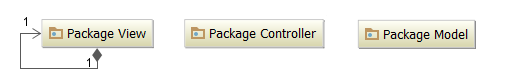
\includegraphics[width=80mm]{../diagrams/classes_packages/classes_packages/packages.png}
    \caption{Diagramme UML de package principale}
    \label{diagram:uml_global}
\end{figure}

\subsection{Mod\`ele (Model)}

\begin{figure}[h]
    \centering
    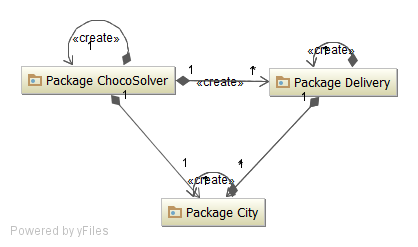
\includegraphics[width=80mm]{../diagrams/classes_packages/classes_packages/model/package_model.png}
    \caption{Diagramme UML du package Model}
    \label{diagram:uml_model}
\end{figure}
\pagebreak

\subsubsection{Mod\`ele Ville (Model.City)}

\begin{figure}[h]
    \centering
    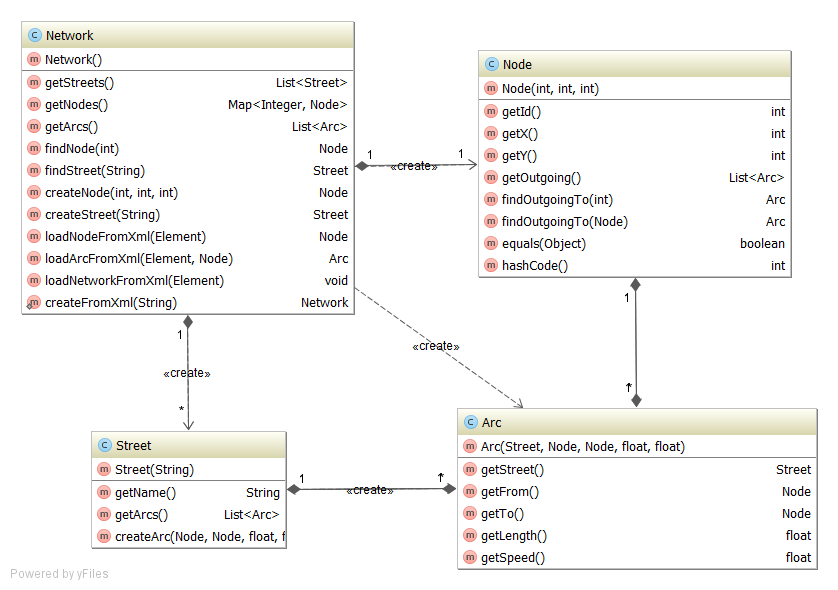
\includegraphics[width=160mm]{../diagrams/classes_packages/classes_packages/model/city.png}
    \caption{Diagramme UML du package Model.City}
    \label{diagram:uml_model_city}
\end{figure}
\pagebreak

\subsubsection{Mod\`ele Livraison (Model.Delivery)}

\begin{figure}[h]
    \centering
    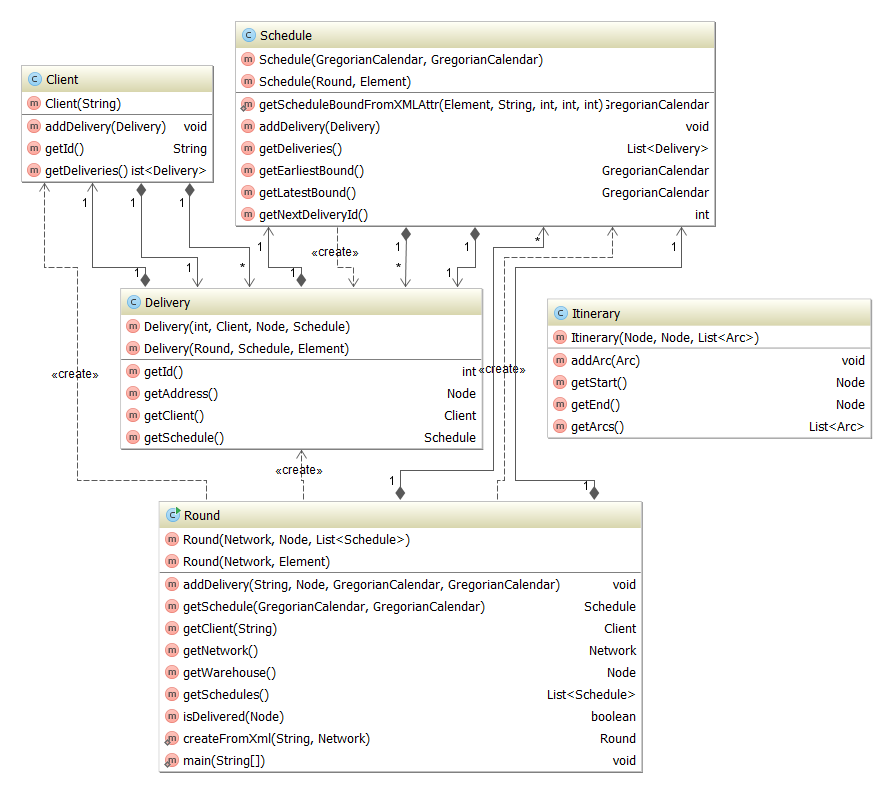
\includegraphics[width=160mm]{../diagrams/classes_packages/classes_packages/model/delivery.png}
    \caption{Diagramme UML du package Model.Delivery}
    \label{diagram:uml_model_delivery}
\end{figure}
\pagebreak

\subsubsection{Mod\`ele Resolution Choco (Model.ChocoSolver)}

\begin{figure}[h]
    \centering
    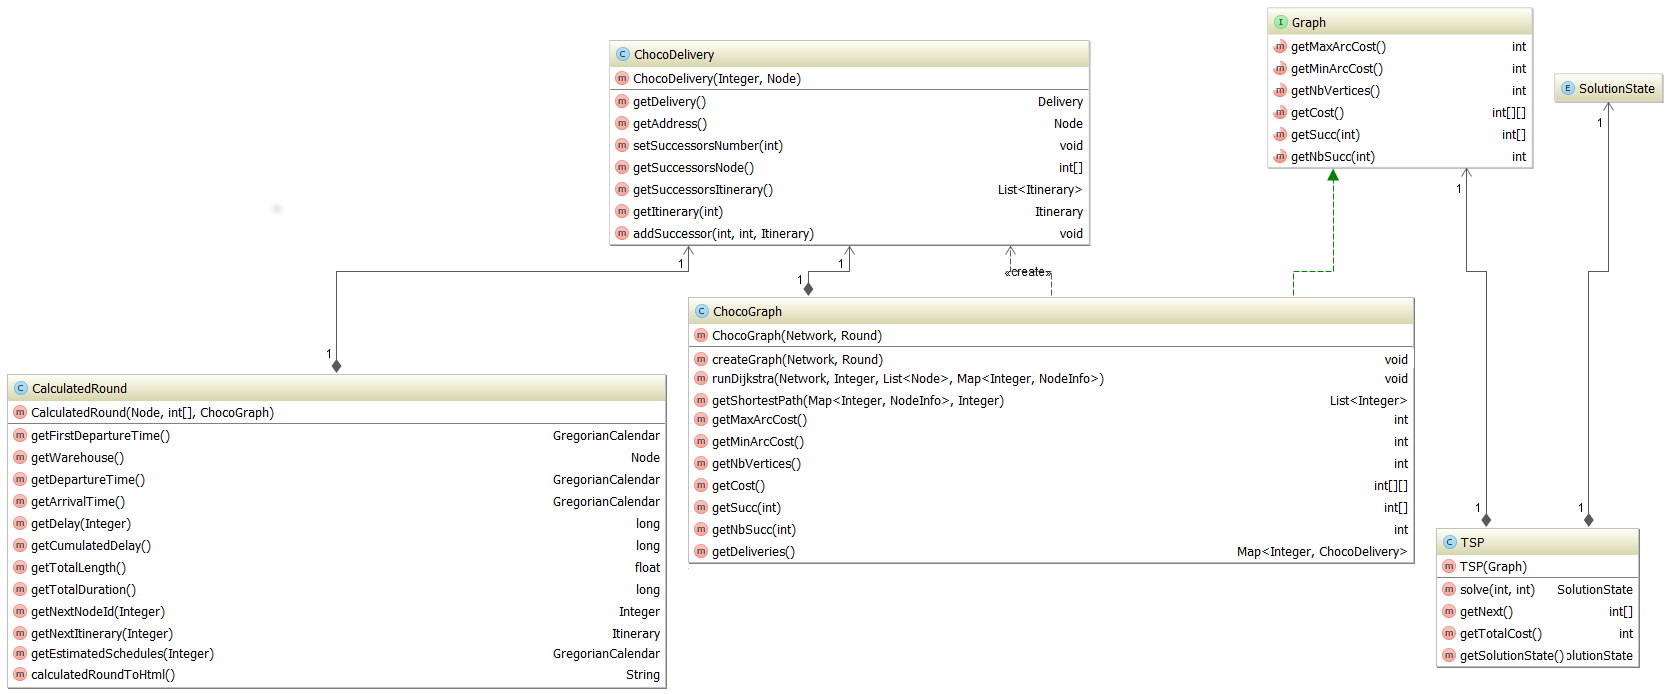
\includegraphics[width=160mm]{../diagrams/classes_packages/classes_packages/model/chocoSolver.png}
    \caption{Diagramme UML du package Model.ChocoSolver}
    \label{diagram:uml_model_choco}
\end{figure}
\pagebreak

\subsection{Vue (View)}

\begin{figure}[h]
    \centering
    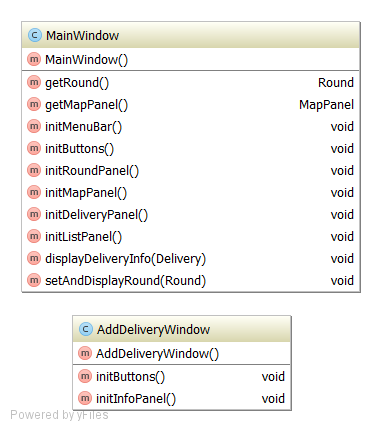
\includegraphics[width=80mm]{../diagrams/classes_packages/classes_packages/view/view.png}
    \caption{Diagramme UML du package View}
    \label{diagram:uml_view}
\end{figure}
\pagebreak

\subsubsection{Vue Carte (View.MapPanel)}

\begin{figure}[h]
    \centering
    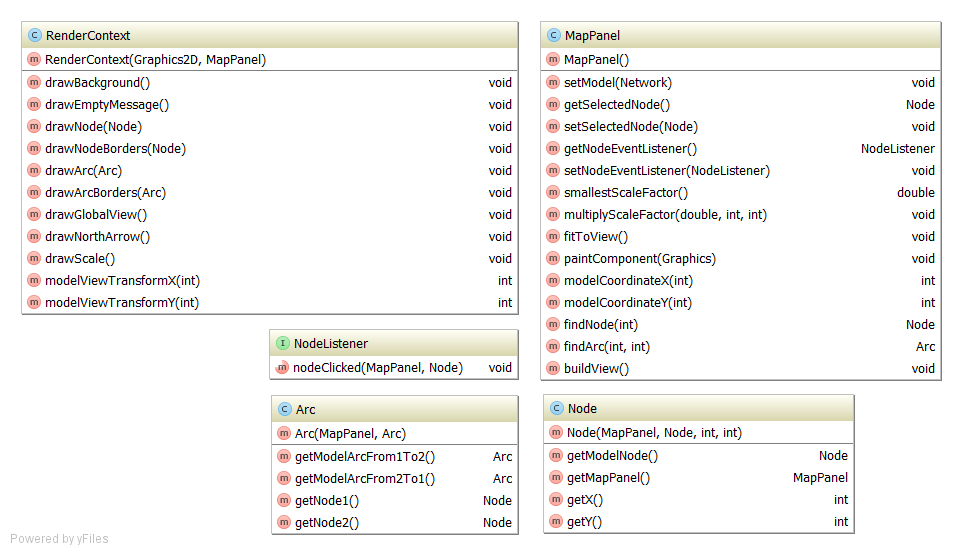
\includegraphics[width=160mm]{../diagrams/classes_packages/classes_packages/view/package_map.png}
    \caption{Diagramme UML du package View.MapPanel}
    \label{diagram:uml_view_map}
\end{figure}
\pagebreak

\subsection{Controlleur (Controller)}

\begin{figure}[h]
    \centering
    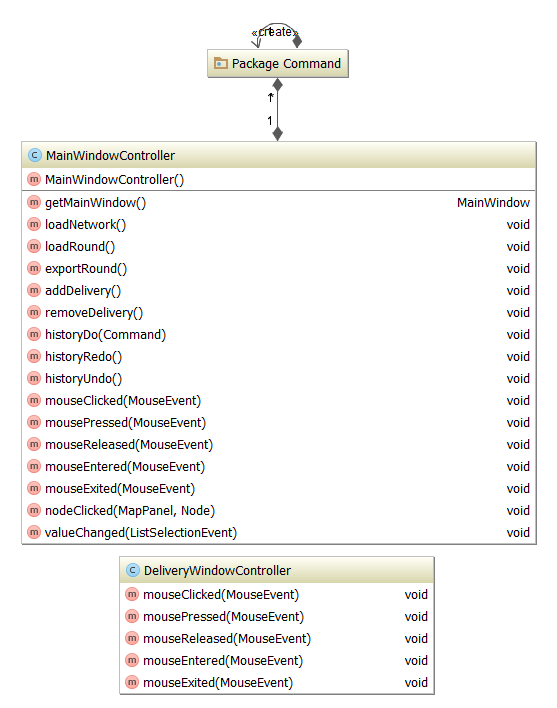
\includegraphics[width=80mm]{../diagrams/classes_packages/classes_packages/controller/controller.png}
    \caption{Diagramme UML du package Controller}
    \label{diagram:uml_controller}
\end{figure}
\pagebreak

\subsubsection{Commande (Controller.Command)}

\begin{figure}[h]
    \centering
    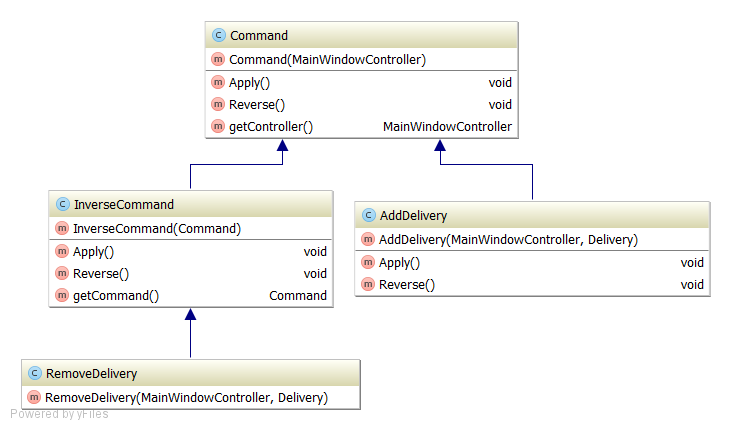
\includegraphics[width=160mm]{../diagrams/classes_packages/classes_packages/controller/package_command.png}
    \caption{Diagramme UML du package Controller.Command}
    \label{diagram:uml_controller_command}
\end{figure}
\pagebreak


% ----------------------------------------------------------------------------- Sequences

\begin{landscape}
    \section{Diagramme de s\'equences}

    \subsection{Chargement d'un tourn\'ee}

    \begin{figure}[h]
        \centering
        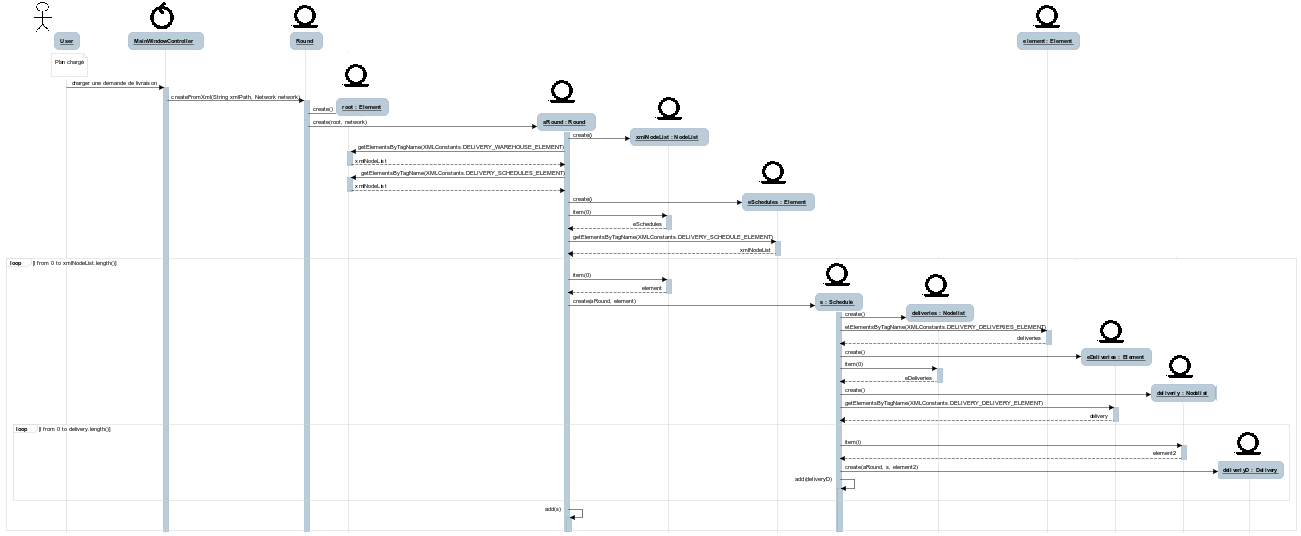
\includegraphics[width=240mm]{../diagrams/sequences/loadRound.png}
        \caption{Diagramme de sequence du chargement de la tourn\'ee}
        \label{diagram:seq_load_round}
    \end{figure}
\end{landscape}
\pagebreak

\begin{landscape}
    \subsection{Calcul d'un tourn\'ee}

    \begin{figure}[h]
        \centering
        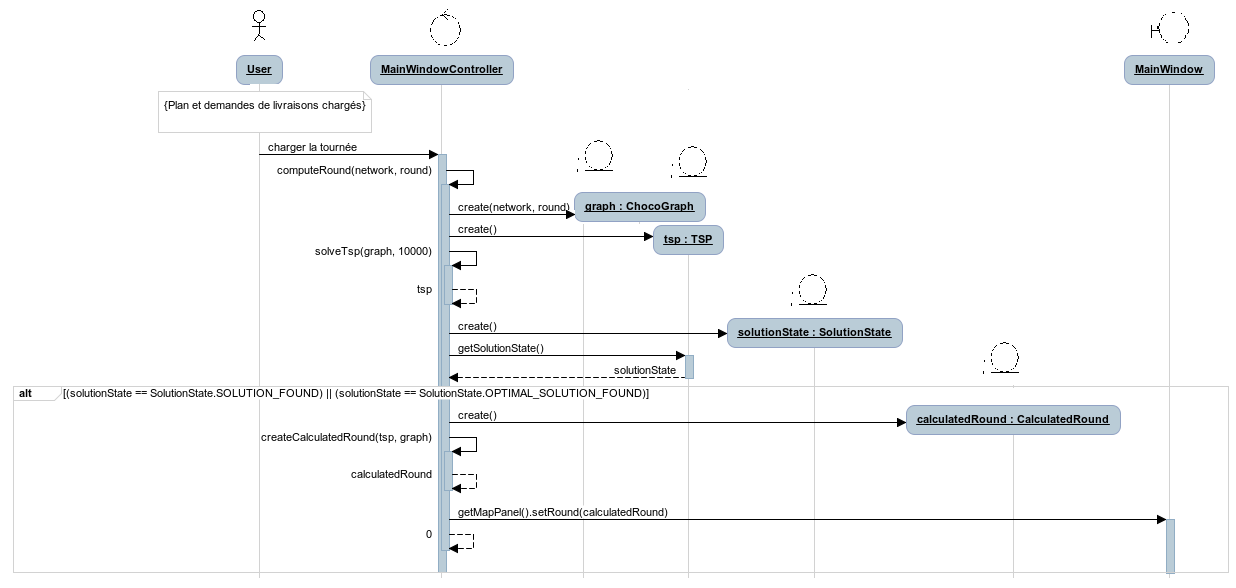
\includegraphics[width=240mm]{../diagrams/sequences/computeRound.png}
        \caption{Diagramme de sequence de calcul de la tourn\'ee}
        \label{diagram:seq_compute_round}
    \end{figure}
\end{landscape}
\pagebreak

\begin{landscape}
    \subsection{Ajout d'une livraison}

    \begin{figure}[h]
        \centering
        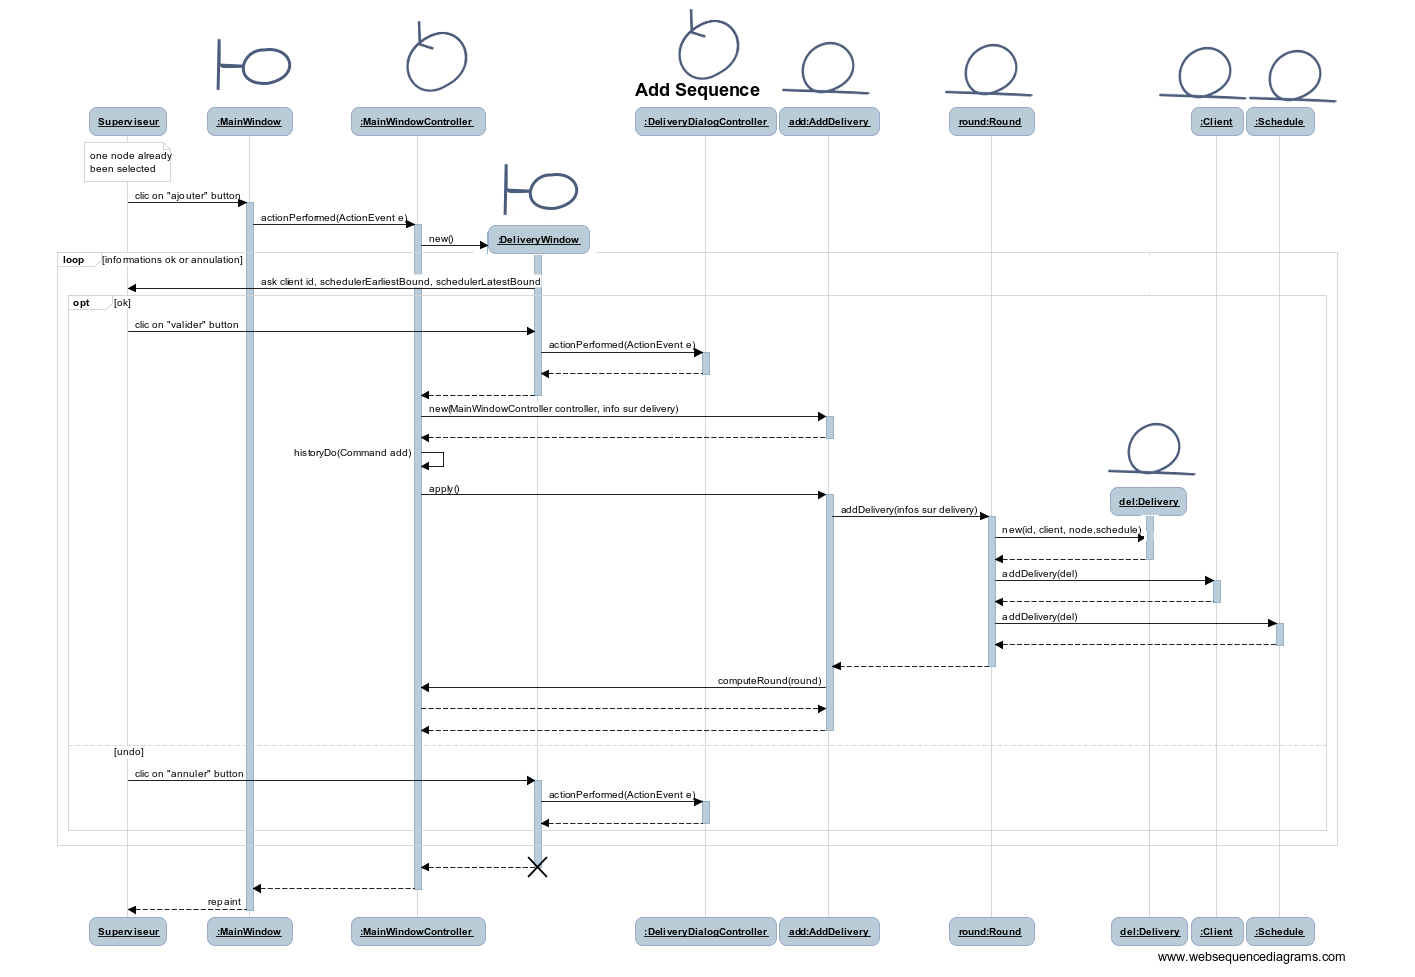
\includegraphics[width=190mm]{../diagrams/sequences/addSequence.png}
        \caption{Diagramme de sequence d'ajout d'une livraison}
        \label{diagram:seq_add_delivery}
    \end{figure}
\end{landscape}
\pagebreak

\begin{landscape}
    \subsection{Suppression d'une livraison}

    \begin{figure}[h]
        \centering
        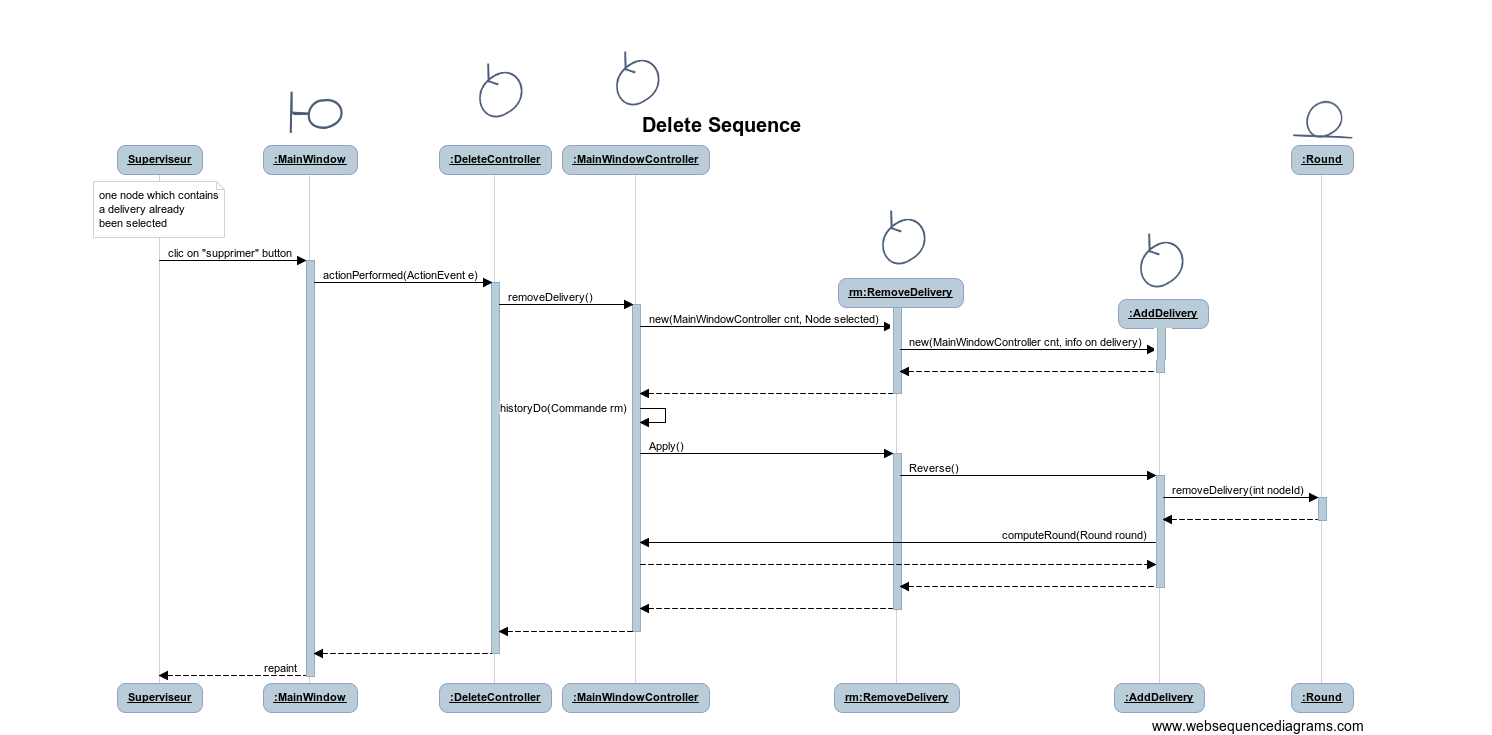
\includegraphics[width=170mm]{../diagrams/sequences/delsequence.png}
        \caption{Diagramme de sequence de suppression d'une livraison}
        \label{diagram:seq_del_delivery}
    \end{figure}
\end{landscape}
\pagebreak

    \chapter{Bilans}
\section{Bilan humain}
\subsection{Méthodologie}
La réalisation du projet Opti\_fret\_COURLY est une occasion idéale pour l’exercice des méthodologies enseignées dans la filière Informatique de l’INSA de Lyon. Celle-ci permit en effet une importante gestion de projet (diagramme de Gantt et de ressources, évaluation des durées des tâches, répartition des rôles, gestion du planning afin de respecter les échéances critiques) et une collaboration entre les différents membres de l’équipe de projet. Ce fut également l’occasion de réaliser un système en collaboration avec un client tenant rôle de maître d’ouvrage, permettant à notre équipe de se rendre compte de l’importance du dialogue avec le client, mais également de la position centrale que doivent occuper ses besoins dans la conception et la réalisation d’une application.

\subsection{Respect du planning et adaptations}
L’efficacité d’une équipe dynamique, sérieuse et bien organisée permit un respect certain des échéances fixées et du planning général. Si, comme escompté, de nombreuses tâches ne purent être effectuées dans le cadre d’une séance de travail, celles-ci furent systématiquement ou presque terminées en dehors des heures pédagogiques.

\subsection{Ressenti}
La première difficulté rencontrée dans la réalisation de ce projet est celle de la continuité du projet IHM. Le projet DevOO semble en effet présenté comme la réalisation du projet précédent, basé sur le même sujet récapitulatif des besoins clients. L'appréhension de nouveaux besoins clients est alors nécessaire.

Il est en outre demandé de réaliser une conception d'application en désaccord avec sa réalisation (diagrammes de cas d'utilisation incluant les applications livreurs et une base de données), ajoutant au sentiment de désarroi de l'équipe de projet.

Enfin, les fichiers XML de description d'un plan et d'une livraison étant livrés sans schéma XML ou DTD associée, la réalisation des parseurs en est approximative et l'exercice de réalisation d'un tel parseur en accord avec une DTD n'est pas pratiqué.
\clearpage

\section{Bilan technique}
\subsection{Sujet}
La réalisation de ce système tire son intérêt majeur du projet réel dont il est issu. Il s’agit en effet là d’une application utilitariste basée sur un cas d’utilisation concret en accord avec les projets futurs que chacun d’entre nous devra réaliser dans un cadre professionnel.

En outre, ce sujet aborde des domaines techniques d'intérêt tels l'affichage graphique d'un graphe interactif, la résolution d'un plus court chemin dans un graphe et la résolution d'un TSP (traveler salesman problem).

\subsection{Compétences acquises}
Ce projet de est en premier lieu l'occasion pour un hexanôme d'approfondir ses compétences en développement dans un langage de programmation de son choix.

Par ailleurs, celui-ci permet la découverte ou l'approfondissement de l'utilisation de bibliothèques graphiques standards dans le cadre du dessin d'un graphe, s'accompagnant de calculs vectoriels et de gestion des événements de la fenêtre parente.

Il en est enfin de même vis-à-vis de l'algorithme de Dijkstra permettant de calculer des plus courts chemins, et de la librairie interfaçant Choco fournie permettant la résolution d'un TSP. L'acquisition et la connaissance du maniement d'une telle librairie sera sans nul doute d'une indéniable utilité dans le cadre de la carrière future de certains membres de notre hexanôme.
\clearpage

    \backmatter
	\phantomsection
	\addcontentsline{toc}{chapter}{\glossaryname}
	\printglossary[title=\glossaryname]
\end{document}
